\documentclass[a4paper,11pt]{article}

\usepackage{../../préambule}

\addtolength{\oddsidemargin}{-0.5cm}
\addtolength{\evensidemargin}{-0.5cm}
\addtolength{\textwidth}{1cm}

\makeatletter
\renewcommand{\maketitle}{%
{\scriptsize colle dans ton cahier d'exercices, et écrit dans ton cahier} \vspace{0.5em}

	\begin{center}
		\LARGE
		\myuline{\@title}
		\vspace{2em}
	\end{center}
}
\makeatother

\usetikzlibrary{shadows,shapes,positioning}

\tikzstyle{shadowtext} = [
	draw=black,
	fill=white,
	rectangle,
	inner sep=10pt,
	style=rounded corners,
	drop shadow={fill=gray,opacity=0.8}
]

\title{Activité : allons aux champs}
\date{}
\author{}

\begin{document}

\maketitle

\begin{vocabulaire}
	Une \textbf{grandeur} est une caractéristique qui se mesure ou se calcule.

	Par exemple le temps, la masse, la taille, le prix...
\end{vocabulaire}

Plusieurs personnes vont dans un magasin de fournitures d'agriculture, afin d'acheter des graines pour leur terrain.

À l'entrée du magasin, on peut voir les exemples suivants : \vspace{2em}

\begin{center}
	\begin{tikzpicture}
		\coordinate (Image1-1) at (6,0);
		\coordinate (Image1-2) at (7,-1);
		\coordinate (Image1-3) at (5,-0.7);
		\node at (Image1-1) {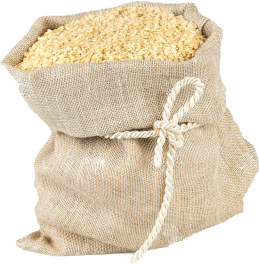
\includegraphics[width=0.2\textwidth]{graines.png}};
		\node at (Image1-2) {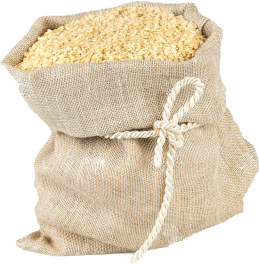
\includegraphics[width=0.2\textwidth]{graines.png}};
		\node at (Image1-3) {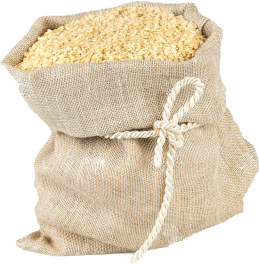
\includegraphics[width=0.2\textwidth]{graines.png}};

		\node [above=2cm,align=flush center] at (Image1-1) {\squared{Terrain de 375m²}};

		\coordinate (Image2-1) at (12,0);
		\coordinate (Image2-2) at (13,-1);
		\coordinate (Image2-3) at (11,-0.7);
		\coordinate (Image2-4) at (12,-1.5);
		\node at (Image2-1) {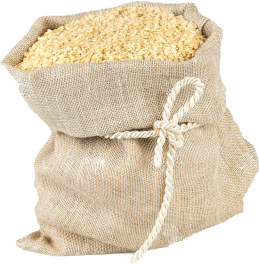
\includegraphics[width=0.2\textwidth]{graines.png}};
		\node at (Image2-2) {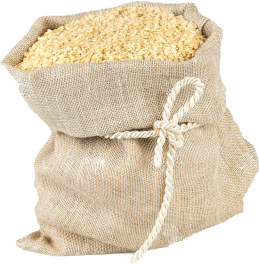
\includegraphics[width=0.2\textwidth]{graines.png}};
		\node at (Image2-3) {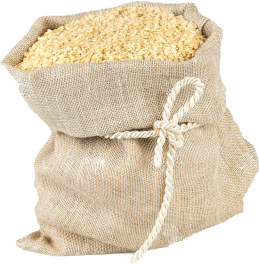
\includegraphics[width=0.2\textwidth]{graines.png}};
		\node at (Image2-4) {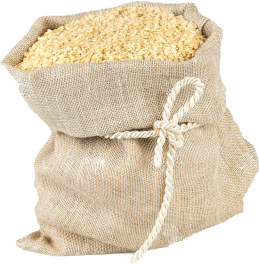
\includegraphics[width=0.2\textwidth]{graines.png}};

		\node [above=2cm,align=flush center] at (Image2-1) {\squared{Terrain de 500m²}};
	\end{tikzpicture}
\end{center}

\begin{itemize}
	\item A l'aide de ces images, réponds au questions suivantes :

	      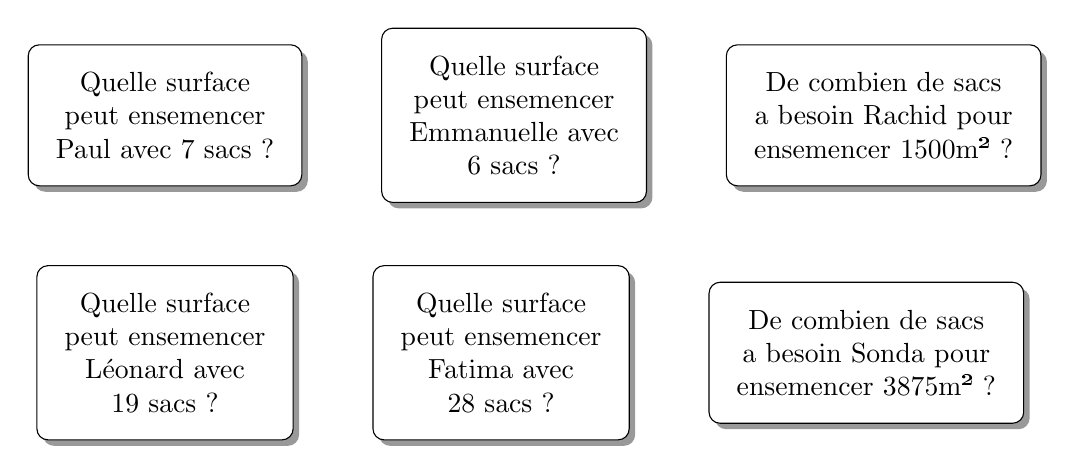
\begin{tikzpicture}
		      \node[shadowtext,align=center] (T1-1) {Quelle surface\\ peut ensemencer\\ Paul avec 7 sacs ?};
		      \node[shadowtext,align=center,right=of T1-1] (T1-2) {Quelle surface\\ peut ensemencer\\ Emmanuelle avec\\ 6 sacs ?};
		      \node[shadowtext,align=center,right=of T1-2] (T1-3) {De combien de sacs\\ a besoin Rachid pour\\ ensemencer 1500m² ?};
		      \node[shadowtext,align=center,below=of T1-1] (T2-1) {Quelle surface\\ peut ensemencer\\ Léonard avec\\ 19 sacs ?};
		      \node[shadowtext,align=center,right=of T2-1] (T2-2) {Quelle surface\\ peut ensemencer\\ Fatima avec\\ 28 sacs ?};
		      \node[shadowtext,align=center,right=of T2-2] (T2-3) {De combien de sacs\\ a besoin Sonda pour\\ ensemencer 3875m² ?};
	      \end{tikzpicture}
	\item Chaque personne aura donc un certain nombre de sacs, et une certaine surface à couvrir. Organise ces données dans un tableau.
	\item En décrivant ta méthode, trouve quelle surface peut être couverte par un sac de graines.
\end{itemize}

\end{document}